        \documentclass{standalone}
        \usepackage{tikz}
        \usetikzlibrary{arrows}
        \usepackage{amsmath}
        \usepackage{amsfonts}
        \begin{document}
        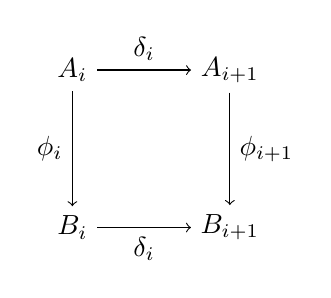
\begin{tikzpicture}

    \node (A1) at (-2,0) {$A_i$};
    \node (A2) at (0,0) {$A_{i+1}$};
    \node (B1) at (-2,-2) {$B_i$};
    \node (B2) at (0,-2) {$B_{i+1}$};
    \draw[->] (A1) -- node[above] {$\delta_i$} (A2);
    \draw[->] (B1) -- node[below] {$\delta_i$} (B2);
    \draw[->] (A1) -- node[left] {$\phi_i$} (B1);
    \draw[->] (A2) -- node[right] {$\phi_{i+1}$} (B2);
        \end{tikzpicture}
        \end{document}
